\chapter{Task: Creating a dominion engine suited for a RL agent} \label{ch:Dominion_engine}
The first step for the project is to create the board game engine which both can be used to play the game of dominion while supporting the playability from a Reinforcement Learning agent. 
Before going into the specifications of the criteria for the engine, the game of Dominion will be explained in short.

\subsection{General rules of the board game Dominion}
Each player starts with a deck of 10 cards, that are identical between players. At the start of each turn, draw 5 cards, at the end of each turn, put all cards from the hand into the discard pile. If there is not enough cards in the deck to draw all 5 cards, then shuffle the discard pile into the deck and draw until 5 cards are drawn. The main goal of the game is to reach terminal state with the most Victory points. These victory points are gained by buying victory cards. 

All cards in the game is categorized into 3 different types of cards. The types are as follows:

\begin{itemize}
    \item Action cards
    \item Treasure cards
    \item Victory cards
\end{itemize}

\textbf{Action cards}:
Action cards are cards that can be played to perform an action, that manipulates the state space in some way or form. A typical example, could be the "smithy" that makes the player draw 3 cards. Based on the price of the

\textbf{Treasure cards}:
These cards have assigned a currency value, which is used to buy other cards. The process of buying a card is discussed later in the rules

\textbf{Victory cards}:
These cards are expensive card, which gives the player victory points. The cards hold no tactical value, other than to be bought to gain victory points.\\\\
A turn consists of an action phase, and a buy phase. The player is granted a single action that the player can do, and a single buy action, which enables the player to buy a single card. It is possible, through, action cards to gain more actions, and more buys. The cards that can be bought are shown as a shared pool of cards that are structured as piles of cards. Every pile represents all the copies of a unique card which can be bought. A typical game setup is shown in the illustration below:\\\\
\begin{figure}[H]
    \centering
    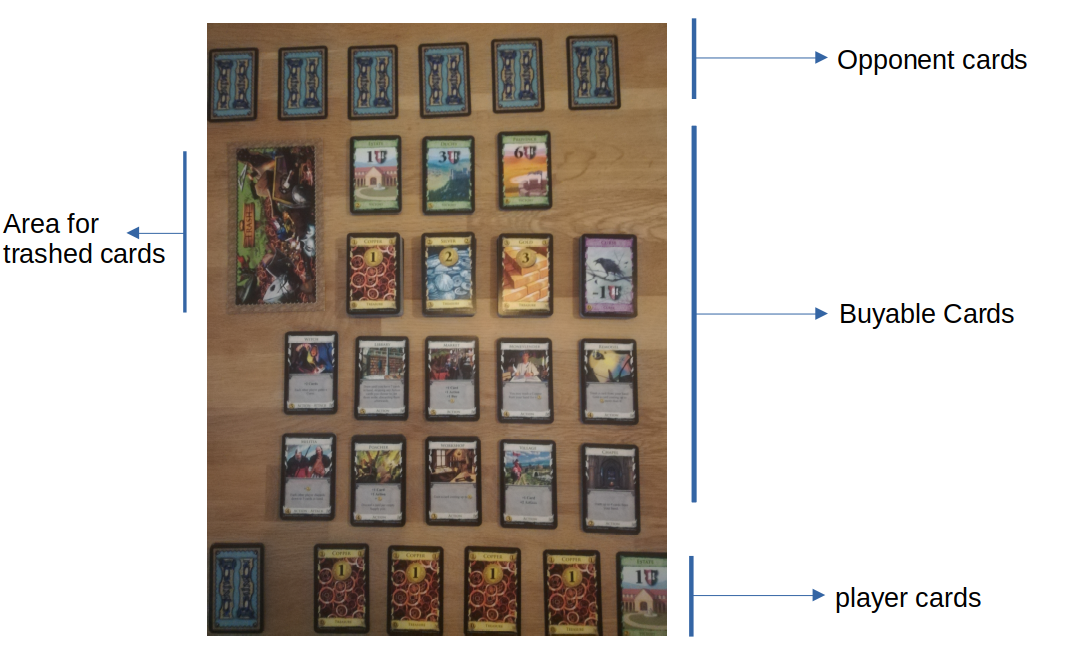
\includegraphics[width=0.9\textwidth]{img/Board_game_setup.png}
    \caption{A typical setup of a Dominion game}
    \label{fig:board_game}
\end{figure}
The usual process is a randomization of the action card piles present. Only 10 action card piles are at play at a time, but around 25 unique action cards exists. For the sake of simplicity, the game will be played with a unique set of cards, that is fixed.\\\\
The process of buying a card in the buy phase, is done by showing the currency in hand that is enough to buy the specified card, and then putting the bought card into the discard pile, so it can be drawn in future turns. The treasure cards used does not disappear, and will be discarded at the end of your turn as all other cards.\\\\
The game ends when the highest cost victory card pile is empty (Card is named "Province"), or when 3 piles of cards are empty. The player with the most victory points wins the game.\\\\


\subsection{Specifications of criteria for the Dominion engine}
The game can be found for free on the internet. Therefore, the reason for creating a new engine, is to have a more flexible engine that supports the use of an AI agent, which does not need to extract information from an image. The advantage of creating a new engine, is that the engine can be designed to ensure that it is capable of giving the entire state space of the game to the AI through a single command call. All actions can also be given to the AI as a list of integers, which the AI must choose from. For the final result of the Dominion game engine, given the nature of the information delivered, it is observed that the game is far more intuitive for the AI than it would be for a human player.

The specific criteria for the Dominion engine are as follows:

\begin{itemize}
    \item The engine must be able to simulate a game of Dominion. (The simulation speed must ideally be faster than the real-time average game length of 20-30 minutes)
    \item The engine must pass a game state object to the agent player, which contains all the information about the current game state.
    \item All actions that can be made in the game must exclusively be run by the agent that is inserted into the game.
\end{itemize}

\subsection{Finished Implementation of the Dominion Engine} \label{sec:engine_implementation}
The finished implementation of the Dominion engine is a python class, which can input arbitrary players and simulate the game. Figure \ref{fig:program structure} shows that structure of the entire progran. Essentially it consists of the Dominion engine, the AI agents, a deck generator and an evaluation program. Figure \ref{fig:Dominion_engine} is the class structure of the Dominion engine. 
\begin{figure}[H]
    \centering
    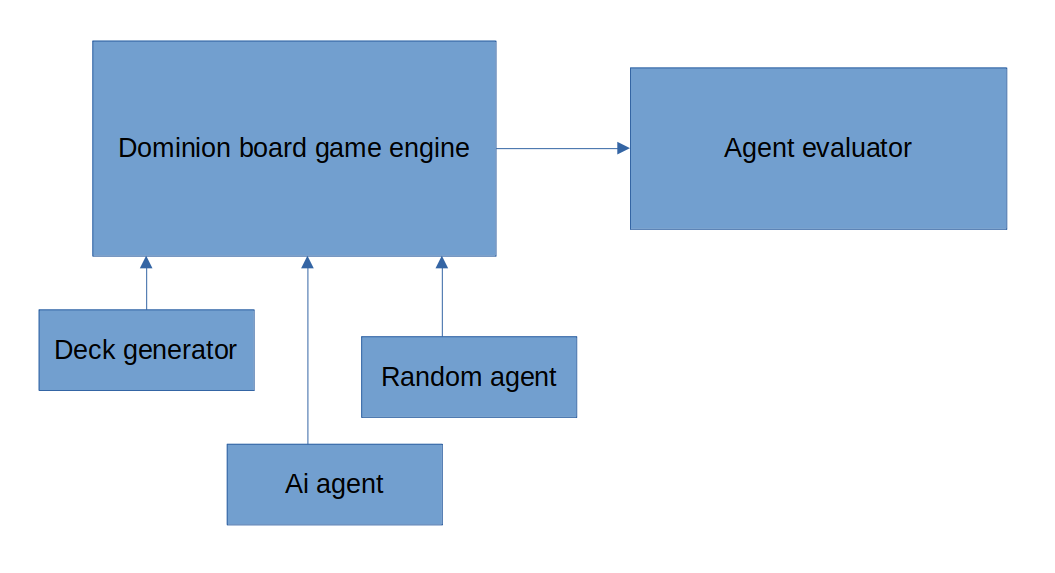
\includegraphics[width=0.8\textwidth]{img/program_structure.png}
    \caption{This is the class structure for the entire project}
    \label{fig:program structure}
    
\end{figure}

\begin{figure}[H]
    \centering
    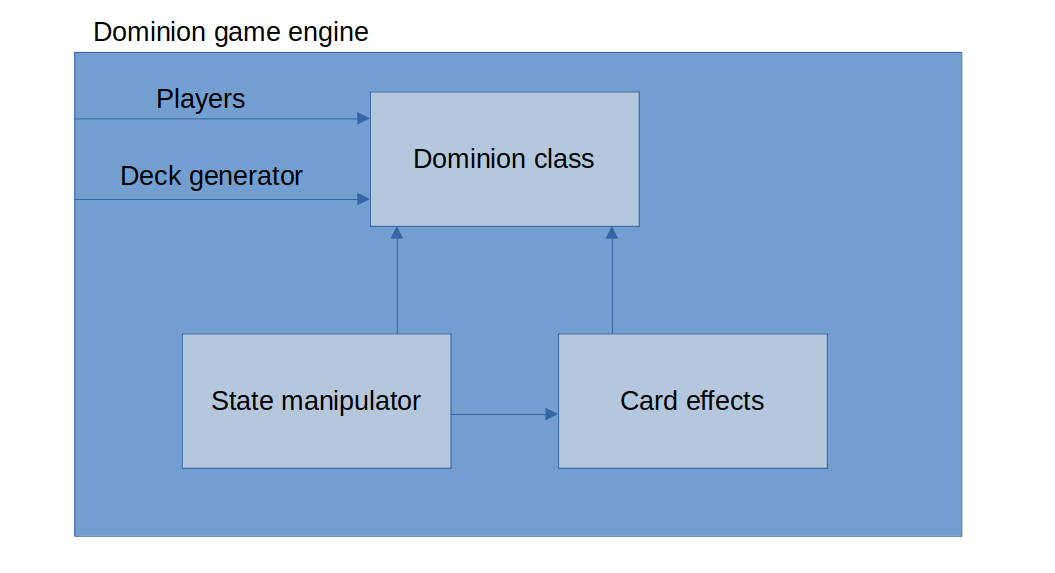
\includegraphics[width=0.8\textwidth]{img/Dominion_game_structure.png}
    \caption{The class structure of the Dominion engine.}
    \label{fig:Dominion_engine}
\end{figure}

The only constriction for the player object, is that the player object must have a function called "choose\_action" with inputs action\_list and game\_state, that returns on of the actions.
The game needs to auxiliary classes, that helps the class compute certain aspects of the game. An entire class has been dedicated to the manipulation of the state object. This might reflect the complexity and size of the programs that is needed to handle the state object.
The card effects class is used to give each card their effect. Each card effect is exclusively limited to effects that alter the state object in some way or form.
An explanation of the gamestate object is as follows:\\
The game state is a dictionary object, which contains the following keys:\\\\
\textbf{game\_state}:
\begin{itemize}
    \item The unique Dominion card set
    \item The supply amount of each card
    \item The type of action that can be done
    \item The parameter that the action needs to be executed
    \item The main player's state
    \item The adversary player's state
\end{itemize}

\textbf{player\_state}:
\begin{itemize}
    \item Player won
    \item Cards in hand
    \item Cards in deck
    \item Known cards on top of deck
    \item Cards in discard pile
    \item Owned cards
    \item Played cards
    \item Action points
    \item Buy points
    \item Treasure value
    \item Victory points
\end{itemize}

It should be observed that each listed key is a unique dimension that the value function must account for. As it is known that there are 17 piles in the game, then the first two keys correspond to 34 dimensions, with approximately 20 values for each. That in itself spans a state space that is 1.71e+44 unique states large. As a normal value function would be too impractical to train, a neural network must be used to approximate the value function. The neural network will be discussed in chapter \ref{ch:neural_networks}.\\\\

An interesting note, is that information regarding the opponent player is partially observable. An example, is that cards in the opponent's hand is not shown, but the amount of cards in the hand is. In the same way, both the order of the cards in the opponent and the player's deck is not shown, but the amount of cards in the deck is.\\\\
Another aspect of the Dominion game, is that since the game only had to support AI agent training, then no GUI is created. This in turn also makes the game go significantly faster than a normal average game. The average game length of the engine using two agents is around 5-10 seconds, instead of 20-30 minutes. The game engine is now ready to be used to train an AI.